\documentclass[11]{article}
%\usepackage{geometry}
\usepackage{graphicx}
\usepackage[pdftex,
bookmarks,
bookmarksopen,
pdfauthor={Mathieu Emily},
pdftitle={GeneGeneInteR}]
{hyperref}

\oddsidemargin -2 mm
\evensidemargin -2 mm
\textwidth 170 mm
\topmargin -2 cm
\textheight 23.5 cm
\newcommand{\code}[1]{\texttt{#1}}
\newcommand{\pkg}[1]{{\fontseries{b}\selectfont #1}}

\usepackage{Sweave}
\Sconcordance{concordance:VignetteGeneGeneInteR.tex:VignetteGeneGeneInteR.Rnw:%
1 42 1 1 2 1 0 1 1 1 2 4 0 2 2 4 0 1 2 3 1 1 2 4 0 1 2 8 1 1 2 4 0 1 2 %
7 1 1 2 4 0 1 2 16 1 1 2 4 0 1 2 2 1 1 2 4 0 1 2 4 1 1 2 4 0 1 2 3 1 1 %
2 4 0 1 2 14 1 1 2 4 0 2 2 4 0 2 2 4 0 1 2 8 1 1 2 4 0 1 2 4 1 1 2 4 0 %
1 2 4 1 1 2 4 0 1 2 24 1 1 2 4 0 1 2 3 1 1 2 4 0 1 2 5 1 1 2 4 0 1 2 10 %
1 1 2 4 0 1 2 12 1 1 2 4 0 1 2 138 1}


\begin{document}
\setkeys{Gin}{width=1.0\textwidth}

%\VignetteIndexEntry{Vignette GeneGeneInteR} 

\title{GeneGeneInteR vignette \\
Gene-based gene-gene interaction analysis in case-controls association studies}
\author{Mathieu Emily \\ AGROCAMPUS OUEST}
\date{\today}
\maketitle
\section{Introduction}
The package \pkg{GeneGeneInteR} aims at providing a collection of statistical methods to search for interaction between genes in case-control association studies. These methods are dedicated to the analysis of biallelic SNP (Single Nucleotide Polymorphism) genotype data. This vignette describes the complete analysis pipeline of a set $ k> 2$ genes, going from data importation to results visualization via data manipulation and statistical analysis.
\vskip1em
In the remainder of this vignette, we illustrate our pipeline through the analysis of a case-control dataset publicly available in the NCBI repository GSE39428 series \cite{Chang:13}. The dataset contains the genotypes of 312 SNPs from 17 genes in a total of 429 patients (266 individuals affected by Rheumatoid Arthritis and 163 Health controls) and is attached to our package \code{GeneGeneInteR} as an external file in the ped format.

\section{Data importation and manipulation}

\subsection{Importation of genotype data}

At first, the path for the files containing genotype data and information regarding the SNP set are loaded:


\begin{Schunk}
\begin{Sinput}
> ped <- system.file("extdata/example.ped", package="GeneGeneInteR")
> info <- system.file("extdata/example.info", package="GeneGeneInteR")
> ## Information about position of the snps
> posi <- system.file("extdata/example.txt", package="GeneGeneInteR")
\end{Sinput}
\end{Schunk}
The importation is performed with the \code{importFile} function:
\begin{Schunk}
\begin{Sinput}
> data <- importFile(file=ped, snps=info, pos=posi, pos.sep="\t")
\end{Sinput}
\end{Schunk}

\vskip1em
The object \code{data} is a list of 3 elements: \code{status}, \code{snpX} (a \code{SnpMatrix} object) and \code{genes.info} (a \code{data.frame}). The \code{status} is available only if the imported format is ped.

\begin{Schunk}
\begin{Sinput}
>  summary(data)
\end{Sinput}
\end{Schunk}

\begin{tabular}{llll}
& Length & Class & Mode \\
status  &      429 & factor   &  numeric\\
snpX  & 133848 & SnpMatrix  & raw \\
genes.info &  4 & data.frame & list
\end{tabular}\\[5mm]

We can check that the \code{snpX} object contains the genotype of 429 individuals for 312 SNPs.
\begin{Schunk}
\begin{Sinput}
> data$snpX
\end{Sinput}
\end{Schunk}

\begin{tabular}{l}
A SnpMatrix with  429 rows and  312 columns\\
Row names:  H97 ... RA345\\
Col names:  rs1002788 ... rs9502656
\end{tabular}\\[5mm]

The \code{genes.info} is a \code{data.frame} with exactly four columns that are named as follows: \code{Chromosome}, \code{Genenames}, \code{ SNPnames} and \code{Position}.
\begin{Schunk}
\begin{Sinput}
> summary(data$genes.info)
\end{Sinput}
\end{Schunk}

\begin{tabular}{lp{0.0001cm}rlp{0.0001cm}rlp{0.0001cm}rlp{0.0001cm}r}
\multicolumn{3}{c}{Chromosome}  &  \multicolumn{3}{c}{Genenames}  &  \multicolumn{3}{c}{SNPnames} & \multicolumn{3}{c}{Position}\\
Min.   &:& 1.000  & PCSK6  &:&74   & rs1002788 &:&  1   & Min.   &:&  7881078  \\
1st Qu.&:& 6.000  & TXNDC5 &:&69  &  rs1005753 &:&  1 &  1st Qu.&:& 11712674\\  
Median &:& 8.000 &  DNAH9  &:&41 &  rs1006273 &:&  1 &  Median &:& 47863803 \\ 
Mean   &:& 9.962 &  CA1    &:&38  & rs10152164&:&  1 &  Mean   &:& 52968484  \\
3rd Qu.&:&15.000 &  VDR    &:&19 &  rs10184179&:&  1 &  3rd Qu.&:& 97191582  \\
Max.   &:&17.000  & Gc     &:&12  & rs1032551 &:&  1  & Max.   &:&123157722  \\
        &&       &   (Other)&:&59  &  (Other)   &:&306 
\end{tabular}


\subsection{Phenotype importation}

Similar to functions introduced to analyze a single pair of genes (see vignette ``Statistical analysis of the interaction between a pair of genes."), the case-control status is stored in a numeric or a factor vector  with exactly two distinct values. If the phenotype is saved in a separate file in table form, it can thus be imported simply by using the \code{read.table} such as for example:

\begin{Schunk}
\begin{Sinput}
> Y <- read.table(system.file("/extdata/response.txt",package="GGItest"),sep=";")
\end{Sinput}
\end{Schunk}
\vskip1em
If the case-control status is provided in the ped file, it can be uploaded as follows:

\begin{Schunk}
\begin{Sinput}
> Y <- data$status
\end{Sinput}
\end{Schunk}

\subsection{Data filtering}

Before performing the statistical analysis, it is very common to remove some SNPs in order to improve the quality of the data. Such a cleaning step can be performed in our \code{GeneGeneInteR} package by using the function \code{snpMatrixScour}. \code{snpMatrixScour} aims at modifying a  \code{SnpMatrix} object by removing SNPs that does not meet criteria regarding the Minor Allele Frequency (MAF), deviation to Hardy-Weinberg Equilibrium (HWE) and the proportion of missing values. In the following example, SNPs with MAF lower than 0.05 or SNPs with p-value for HWE lower than 0.001 or SNPs with a call rate lower than 0.9 are removed from the object \code{data}.

\begin{Schunk}
\begin{Sinput}
> data <- snpMatrixScour(data$snpX,genes.info=data$genes.info,min.maf=0.05,min.eq=1e-3,call.rate=0.9)
\end{Sinput}
\end{Schunk}

\vskip1em
The following lines show that the dataset now contains only 209 SNPs, meaning that 103 SNPs have been filtered out.

\begin{Schunk}
\begin{Sinput}
> data$snpX
\end{Sinput}
\end{Schunk}

\begin{tabular}{l}
A SnpMatrix with  429 rows and  209 columns\\
Row names:  H97 ... RA345 \\
Col names:  rs10510123 ... rs4328262
\end{tabular}

\vskip1em
Since the use of stringent filters could lead to the elimination of all SNPs within a gene, care has to be taken during the filtering step. However, in such a situation the gene without SNPs is removed from the dataset and a warning message is provided for the user.

\vskip1em
In other situations, the user might be interested in performing the analysis on a predefined subset of SNPs. For that purpose, the \code{select.snps} function provides three options to extract of collection of SNPs by specifying the argument \code{select} that should be one of the following:

\begin{itemize}
\item a numeric vector with only the column number in the snpMatrix (or row number for genes.info) of each selected SNP. The following line allow the extraction of the 10 first SNPs:
\begin{Schunk}
\begin{Sinput}
> selec <- select.snps(data$snpX, data$genes.info, select=1:10)
\end{Sinput}
\end{Schunk}
\item a character vector with the names of each selected SNP or each selected gene. The following example is used to extract genes DNAH9 and TXNDC5:
\begin{Schunk}
\begin{Sinput}
> selec <- select.snps(data$snpX, data$genes.info, c("DNAH9","TXNDC5"))
\end{Sinput}
\end{Schunk}
\item a character vector which elements are position bounds of genes. Each element of the vector is either of the form "begin:end", or "chr:begin:end" if you have to precise the chromosome of the gene. The following code allow to select SNPs from position 101342000 to 101490000 on chromosome 15:
\begin{Schunk}
\begin{Sinput}
> selec <- select.snps(data$snpX, data$genes.info, c("15:101342000:101490000"))
\end{Sinput}
\end{Schunk}
\end{itemize}

\subsection{Imputation}

Since our pipeline of analysis does not handle with missing values, SNPs filtering as well as SNPs selection can help removing missing data. This can be done easily by applying the \code{snpMatrixScour} with \code{call.rate=1} argument. However, in that case, SNPs with an acceptable call rate are also removed and the lost information is likely to be critical.  Genotype imputation is then commonly performed to keep most of the informative SNPs in the dataset. Since our genotype data are stored into \code{SnpMatrix} object, we implement the  \code{imputeSnpMatrix} function that wraps  \code{snp.imputation} and \code{impute.snps} functions from \code{snpStats} package. Our \code{imputeSnpMatrix} function mimics a Leave-One-Out process where missing SNP are imputed for an individual based on a model trained on all other individuals.

\vskip1em
In our example, the following lines show that after the filtering step, 844 missing values still remain in the dataset.

\begin{Schunk}
\begin{Sinput}
> sum(is.na(data$snpX))
\end{Sinput}
\end{Schunk}
\code{[1] 844}

\vskip1em
To impute those missing values, we simply used our \code{imputeSnpMatrix} function as follows:

\begin{Schunk}
\begin{Sinput}
> data <- imputeSnpMatrix(data$snpX,data$genes.info)
\end{Sinput}
\end{Schunk}
\code{|----------------------------------------------------------| 100\%}

\vskip1em
A simple check of the dataset show that all missing values have been imputed:

\begin{Schunk}
\begin{Sinput}
>  sum(is.na(data$snpX))
\end{Sinput}
\end{Schunk}
\code{[1] 0}


\vskip1em
When the amount of missing values is so important that \code{snp.imputation} is not able to find a rule of imputation, some missing values may remain. In that case, the user can specify the action to be done thanks to the \code{om.rem} arguments:
\begin{itemize}
\item \code{om.rem="none"}: leave the dataset as it is,
\item \code{om.rem="SNP"}: remove all SNPs with remaining missing values,
\item \code{om.rem="ind"}: remove all individuals with remaining missing values.
\end{itemize}

\vskip1em
It is noteworthy that removing all SNPs is often more parsimonious than removing individuals and allows to get a dataset without any missing values with minimum information-loss.

\vskip1em
Although, function \code{snp.imputation} can calculate accurate rules for imputation, we encouraged the user to first input missing genotype with an external software (such as IMPUTE2 \cite{Howie:09}) prior to the importation step. 

\section{Statistical analysis}

The statistical analysis of a set of genes, as implemented in the \code{GGI} function, consists in performing all possible pairwise tests between two genes. Pairwise tests are conducted by using the \code{method} argument with one of the ten method detailed in the vignette ``Statistical analysis of the interaction between a pair of genes." The \code{GGI} function takes two further mandatory arguments: \code{Y} the vector of case-control status and \code{snpX}, a \code{SnpMatrix} object that store the genotypes for all SNPs. It is assumed that SNPs within the same gene are consecutive in the \code{snpX} argument. Furthermore, gene information, such as gene ordering and the number of SNPs within each gene, has to be provided either in the \code{genes.length} or in the \code{gene.info} argument.

\vskip1em
\noindent
The following line allow the computation of all pairwise tests between the 17 genes of our example dataset with the PCA-based method.

\begin{Schunk}
\begin{Sinput}
> GGI.res <- GGI(Y=Y, snpX=data$snpX, genes.info=data$genes.info,method="PCA")
\end{Sinput}
\end{Schunk}
\vskip1em
\noindent
The output of the \code{GGI} function is a an object of class \code{GGInetwork}.

\begin{Schunk}
\begin{Sinput}
> class(GGI.res)
\end{Sinput}
\end{Schunk}
\code{[1] "GGInetwork"}

\vskip1em
\noindent
The class \code{GGInetwork} is an S3 class based on a list of 4 elements \code{statistic}, \code{p.value}, \code{method} and \code{parameter}. When \code{method="PCA"} a fifth element is added to the \code{GGInetwork} object \code{df}. 

\begin{Schunk}
\begin{Sinput}
> names(GGI.res)
\end{Sinput}
\end{Schunk}
\code{[1] "statistic" "p.value"   "df"        "method"    "parameter"}

\vskip1em
\noindent
Elements \code{statistic}, \code{p.value} and \code{statistic}, \code{df} are squared matrices with $M$ rows and $M$ columns where $M$ is the number of genes in the dataset. The general terms of each matrices are respectively the statistic, the p-value and the degrees of freedom of the Likelihood Ratio Test. The element \code{method} is the name of the method used to perform the pairwise interaction tests. Finally, the element \code{parameter} is a list of the parameters used to perform the pairwise interaction tests.

\vskip0.5em
\noindent
As example, the \code{GGI.res} object generated in the previous example is a list of 5 elements. Each cell of the output \code{p.value} matrix is the p-value of the corresponding pairwise test. The pairwise p-values obtained for the 4 first genes (bub3, CA1, CDSN, DNAH9) of our dataset can be observed as follows:


\begin{Schunk}
\begin{Sinput}
> round(GGI.res$p.value[1:4,1:4],digits=4)
\end{Sinput}
\end{Schunk}
\begin{tabular}{lrrrr}
&        bub3  &  CA1 &  CDSN & DNAH9\\
bub3  & 0.0000 & 0.1684 & 0.3179 & 0.1851\\
CA1 &  0.1684 & 0.0000 & 0.0697 & 0.0000\\
CDSN & 0.3179 & 0.0697 & 0.0000 & 0.4539\\
DNAH9 & 0.1851 & 0.0000 & 0.4539 & 0.0000
\end{tabular}


\vskip1em
\noindent
Significant results can be summarized using the S3 method \code{summary} for class \code{GGInetwork}. The method \code{summary} prints the pairs of genes with a interaction p-value lower than $0.05$ after (1) no correction (2) a bonferroni correction and (3) Benjamini \& Hochberg correction for multiple testing.

\begin{Schunk}
\begin{Sinput}
> summary(GGI.res)
\end{Sinput}
\end{Schunk}

\code{Gene-gene interaction network of  17  genes performed with:\\ 
\null \hskip5em 	 Principal Component Analysis}

\code{Significant interaction with no correction at the level of 0.05}

\code{-------}

\begin{tabular}{lrrrr}
& Gene1    &Gene2& Uncorrected p-value\\
1   & TXNDC5   &   VDR&             8.9e-10\\
2    & DNAH9   &TXNDC5&             1.9e-09
\end{tabular}


\code{$\vdots$}

\code{Significant interaction with a bonferroni correction at the level of 0.05}

\code{-------}

{\tt
\begin{tabular}{lrrrr}
&Gene1 &   Gene2 & bonferroni p-value\\
1  &TXNDC5  &    VDR     &       1.2e-07\\
2   &DNAH9 &  TXNDC5     &       2.6e-07
\end{tabular}
}

\code{$\vdots$}

\code{Significant interaction with a Benjamini \& Hochberg correction at the level of 0.05}

\code{-------}

{\tt
\begin{tabular}{lrrrr}
&    Gene1 &   Gene2 & BH p-value\\
1 & TXNDC5 &     VDR  &  1.2e-07\\
2  & DNAH9  & TXNDC5  &  1.3e-07
\end{tabular}
}
\section{Visualization}

The visualization of the results can be performed with the S3 method \code{plot} for class \code{GGInetwork}. Given a \code{GGInetwork} object obtained from the analysis of $M$ genes with our \code{GGI} function, results can be visualized through two types of representation: an heatmap-like visualization with the \code{method="heatmap"} argument and a network-like representation with the \code{method="network"} argument. 

\subsection{Heatmap-like visualization}\

\noindent
The \code{plot} method can be simply used with the \code{GGInetwork} object as the single input argument. Figure~\ref{Fig:GGIPlotD} (a) and (b) show the graphical representation where all pairwise interactions are plotted (Fig. \ref{Fig:GGIPlotD} (a)) or only the interaction between the 3 genes CA1, Gc and PADI1 with the argument \code{genes} (Fig. \ref{Fig:GGIPlotD} (b)).

\begin{figure}[h!]
\begin{center}
\begin{tabular}{cc}
(a) \code{R> plot(GGI.res)} & (b) \code{R> plot(GGI.res,genes=c("CA1","Gc","PADI1"))} \\
\\
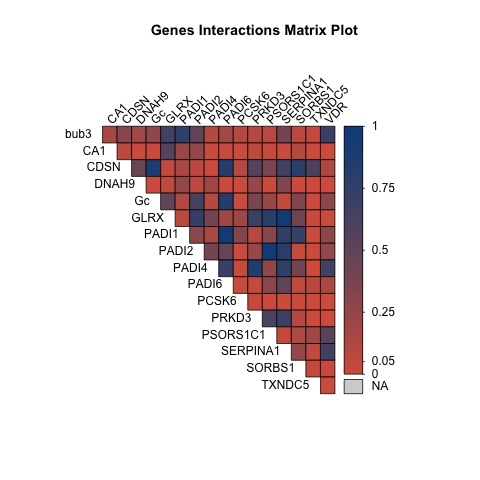
\includegraphics[width=5cm]{GGIPlot1} & 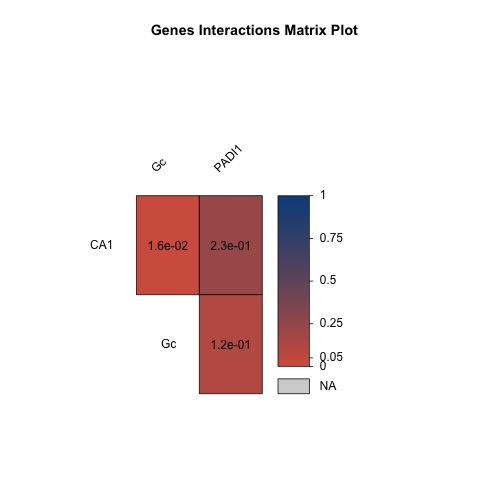
\includegraphics[width=5cm]{GGIPlot2}
\end{tabular}
\end{center}
\caption{\label{Fig:GGIPlotD} Default output of the function \code{GGI.plot} considering (a) the whole set of genes or (b) a restricted set of 3 genes.}
\end{figure}

\noindent
When the number of genes is below 15, p-values and names are drawn to make matrix reading easier (see Figure~\ref{Fig:GGIPlotD}(b)). However, when the number of genes is larger than 15, p-values are not drawn and gene names are kept while if the number of genes is larger than 25, none of the lvalues or the gene names are displayed  (see Figure~\ref{Fig:GGIPlotD}(a)). In that case, the default behavior of the function is to start an interactive process where user can click on a cell of interest to open a tooltip displaying which genes are involved in the selected interaction and the p-value of the interaction test. Tooltips can be closed if user clicks anywhere else than on a cell. This process stops when the user presses the escape button (or terminates the locator procedure in general) or when the user clicks on any place other than a cell when no tooltip window is open. 

\vskip1em
\noindent
Several arguments can further be specified to customize the output graphics such as colors (arguments \code{col} and \code{NA.col}), width of the bar for colors (argument \code{colbar.width}),  and titles (argument \code{title}). User can also  decide whether p-values (argument \code{draw.pvals}) and gene names (argument \code{draw.names}) should be drawn and is allowed to disable the interactivity of plot (argument \code{interact}). To further improve plot clarity and hence allowing a better interpretation of the results, (1) genes can be ordered according to a hierarchical clustering (argument \code{hclust.order}), (2) p-values can be reported in -log10 scale (argument \code{use.log}) and (3) a threshold can be applied to the p-values in order to distinguish between significant and non-significant interactions (argument \code{threshold}).

\vskip1em
\noindent 
Figures~\ref{Fig:GGIPlotCustom1} and \ref{Fig:GGIPlotCustom2} provide two plots resulting from different sets of arguments passed to the \code{plot} function.


\begin{figure}[!h]
\code{R> plot(GGI.res,col=c("black","cyan","white"),colbar.width=0.25,title="Interaction between 17 genes",hclust.order=TRUE,use.log=TRUE,threshold=NULL,NA.col ="\#D3D3D3",draw.pvals=FALSE,draw.names=TRUE,interact=FALSE)}
\begin{center}
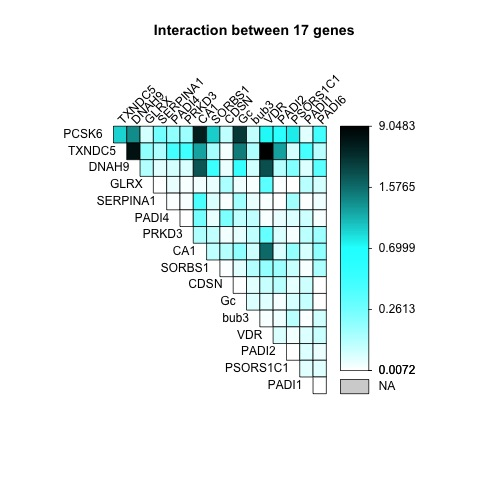
\includegraphics[width=8cm]{GGIPlot3}
\end{center}
\caption{\label{Fig:GGIPlotCustom1} Example of the use of \code{plot} arguments when no threshold is applied to the p-values.}
\end{figure}


\begin{figure}[!h]
\code{R> plot(GGI.res,col=c("black","cyan","white"),colbar.width=0.05,title="Interaction between 17 genes",hclust.order=TRUE,use.log=FALSE,threshold=0.05,NA.col ="\#D3D3D3",draw.pvals=FALSE,draw.names=TRUE,interact=FALSE)}
\begin{center}
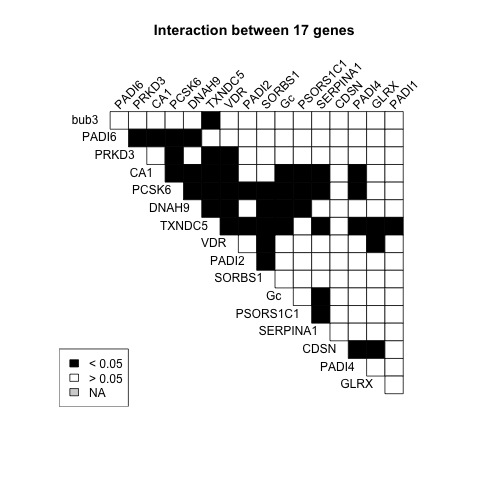
\includegraphics[width=8cm]{GGIPlot4}
\end{center}
\caption{\label{Fig:GGIPlotCustom2} Example of the use of \code{plot} arguments when a threshold of $0.05$ is applied to the p-values.}
\end{figure}

\newpage
\null
\newpage


\subsection{Network-like visualization}

\noindent 
The \code{plot} function with \code{method="network"} aims at drawing a graph between genes where two genes are adjacent if the pvalues between these two genes is below a given threshold (argument \code{threshold} with a default value equal to $0.05$). The display of the network is performed by utilizing  the \code{graph\_from\_data\_frame} from the \code{igraph} R package \cite{Csardi:06}.

\vskip1em
\noindent
Two additional arguments can be used to customize the network. First, user can focus on a specific subset of genes with the argument \code{genes} and secondly, gene(s) not linked to other genes can be removed from the graph with argument \code{plot.nointer}.

\vskip1em
\noindent
Figure~\ref{Fig:NetworkD} displays the default network obtained with all genes. In figure~\ref{Fig:NetworkC}, a subset of only 12 genes have been selected to be the vertices of the graph. However, genes bub3 and PADI1 does not have a pvalue below the threshold of 0.05 with any of the other selected genes. Since the argument \code{plot.nointer} is set to \code{TRUE}, the two genes bub3 and PADI1 are not drawn in the resulting network.


\begin{figure}[!h]
\code{R> set.seed(1234)\\
  R> plot(GGI.res,method="network")}
\begin{center}
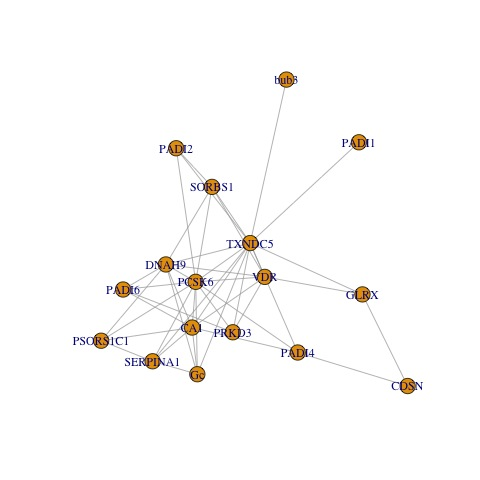
\includegraphics[width=10cm]{network}
\end{center}
\caption{\label{Fig:NetworkD} Default output of \code{draw.network}}
\end{figure}

\newpage

\begin{figure}[!h]
\code{R> set.seed(1234)\\
  R> plot(GGI.res,method="network",genes=c("bub3","CDSN","Gc","GLRX","PADI1","PADI2","PADI4",\\ 
                                           \null \hskip5em"PADI6","PRKD3","PSORS1C1","SERPINA1","SORBS1"),\\
          \null \hskip5em threshold=0.05,plot.nointer=FALSE)}
\begin{center}
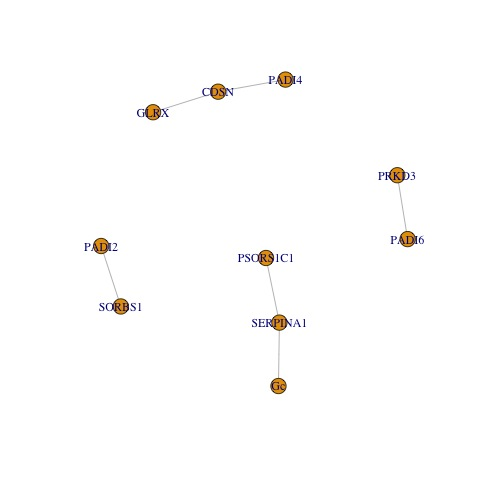
\includegraphics[width=10cm]{networkCust}
\end{center}
\caption{\label{Fig:NetworkC} Output of \code{draw.network} with a customized set of arguments.}
\end{figure}

\newpage

\section{References}
\bibliographystyle{alpha}
\bibliography{Biblio}

\end{document}
